\section{Metode}
\subsection{Overordnet system design}
\begin{figure}[H]
    \centering
    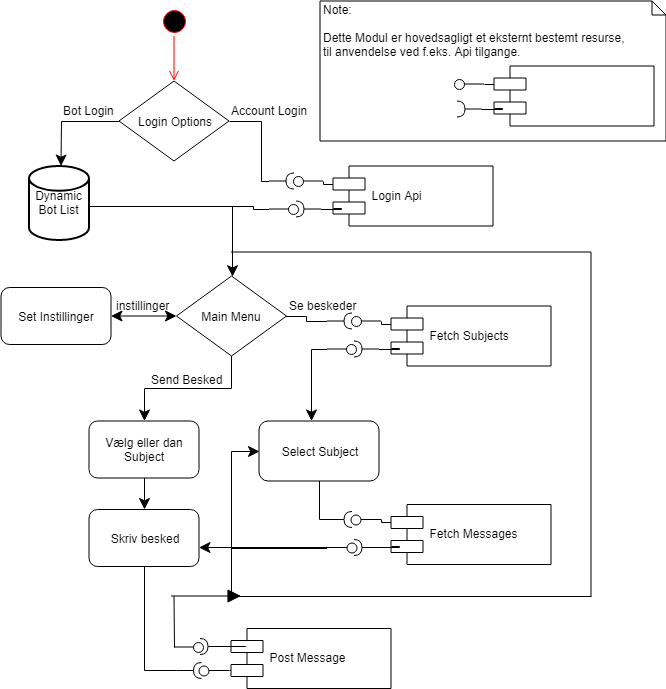
\includegraphics[width=0.75\linewidth]{Projectdoc/Assets/Illustrationer/system-diagram.png}
    \caption{System aktiverings diagram}
    \label{fig:sysdiagram}
\end{figure}

Systemet beskrevet ved [Figur \ref{fig:sysdiagram}] er hovedsageligt designet efter et User Activated Action Event Flow. 
Dette vil sige at alle systemets aktiviteter er baseret på en brugers aktive handlinger, og kan derved styres fra et centralt sted. Her tales om enten brugerens egen enhed, eller en central system server, der kun responderer på brugerens kommandoer.
En af de store fordele ved at have en central server, i modsætning til brugernes enhed som håndtering, er den markant større mulighed for lokalt server arbejde. På en central server er der mulighed for at forebygge heavy-load og f.eks. indlæse, samt gemme (som en slags cache), alle beskeder for en specifik tråd, inden brugeren faktisk beder om dens indhold. Derved kan man benytte serverens hviletilstand til aktivt at forebygge aktiviteter, og derved mindske fremtidige belastnings problemer.

\begin{figure}[H]
    \begin{subfigure}{0.5\textwidth}
        \centering
        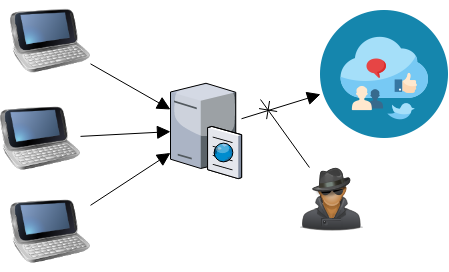
\includegraphics[width=1\linewidth, height=4cm]{Projectdoc/Assets/Illustrationer/Security_diagram_1.png} 
        \caption{Central server}
        \label{fig:central_server}
    \end{subfigure}
    \begin{subfigure}{0.5\textwidth}
        \centering
        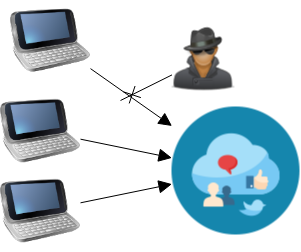
\includegraphics[width=0.7\linewidth, height=4cm]{Projectdoc/Assets/Illustrationer/Security_diagram_2.png}
        \caption{Client-baseret system}
        \label{fig:decentral_server}
    \end{subfigure}
    \caption{Forskellen på central og decentral server struktur}
    \label{fig:serverstruktur}
\end{figure}

En central server trods dens eventuelle positive effekter, er dog også et generelt større sikkerhedsbrud. F.eks. Kunne en sådan server, (Illustreret ved [Figur \ref{fig:central_server}]), lække generelle lagerede informationer, eller lige frem enten blive overvåget for kommunikation, samt blive spærret som en helhed. Dette vil selvfølgelig også kunne ske for den enkelte bruger [\ref{fig:decentral_server}], men disse ville i sådanne tilfælde også kun påvirke den enkelte, og ikke systemet som en helhed.\\
Grundet disse negative effekter for en central server, der generelt berører brugerens sikkerhed, vil den mest optimale løsning for projektets sikre kommunikation være, at anvende brugernes enkelte enheder til system håndtering. Dette vil dog ikke i sig selv kunne tages til konklusion, da et system baseret alene på enkelte enheder egen håndteringer, vil kunne danne en større kompromitterings fare. Denne fare vil kunne opstå ved anvendes af lokalt cache for data fetching, da denne information vil kunne findes på flere nodes, dog uden denne cache vil de enkelte enheder skulle foretage mange heavy loads forespørgsler. Disse forespørgsler vil ikke bare danne større spekulation hos netværksmonitorering, og derved en større sandsynlighed for terminering, men også danne et meget stort dataforbrug hos enddevices, samt en lang load time, der kan fremprovokere brugerfejl.

% foruden selve strukturen:
% Er der også problemer med fetching af sammenhæng.

% Tilsidst:
% Kan der være et kulturelt problem i steganografi på et socialt medie.

\subsection{Teori}
Top

\subsubsection{API struktur / Socket kommunikation}
% Hvad er Api struktur ? Hvorfor bruger man APIer? REST og CRUD beskrivelse
% Hvad er socket kommunikation ?

\subsubsection{Caching}

\subsubsection{Decentralisering}
For at holde den samlede kommunikationsplatform så sikkert, og pålideligt, som muligt, vil mulighederne for decentralisering af systemet blive diskuteret i dette afsnit.
Det grundlæggende princip er, at jo mere et givet system afhænger af bestemte nodes, jo mere sårbart vil det også være. På den anden side, vil anvendelsen af servere i centralt systemet også tillade en langt højere effektivitet. Derfor vil forskellige aspekter af kommunikationsplatformen blive diskuteret for at kunne finde et kompromis mellem helt centraliseret og helt decentraliseret.

For at kunne opretholde en mængde af bots, her værende dummy brugere som sikrer anonymitet for brugeren, associeret med en potentielt mistænkelig opførelse, vil det være nødvendigt at kunne tilføje nye bots til netværket løbende, samt opdatere status af nuværende bots, da denne type bots har været lukket ned på flere sociale medier. Én mulig løsning på dette problem kunne være at holde en database opdateret med statussen af de enkelte bots. Hvis en given bot så blev lukket ned, ville den opdaterede database, gøre enhver bruger i stand til blot at vælge en anden bot. Problemet med denne løsning er, at den vil introducere et svagt link, databasen selv, der ville gøre en væsentlig del af systemet ubrugeligt, hvis den blev taget ned, indtil en erstatning kunne sættes op. Såfremt denne database kun kontaktes for at få listen opdateret, vil trafikken imellem den og klienterne dog være begrænset. Man kunne også forestille sig en ekstra database, som kun vil blive kontaktet hvis den primære er inaktiv, og at denne database kender til andre databaser som er backups af den primære. Denne opbygning vil gøre det meget svært at lukke systemet i længere tid.
% Så længe den primære anvendelse af systemet foregår igennem en hjemmeside, vil denne server kunne sidde med denne bot liste selv. Dette gør dog blot denne server endnu mere kritisk.
En måde at undgå dette databaseproblem, er at lade hver klient have en lokal liste over aktive bots. Denne liste vil så med jævne intervaller blive opdateret igennem klient opdateringer. Med denne fremgang er det tænkeligt, at systemet vil kræve mange opdateringer, eller at der ofte vil være et antal utilgængelige bots på listen. 
% Denne liste kunne også findes på en database som udelukkende har denne liste af bots. Dette vil minimere trafikken til databasen, hvilket vil mindske dens synlighed.


% Ingen interconnectivity mellem devices, men skal facilitere data udveksling.... How the f-ing hell?

% Blockchain, ha lol (det ville kunne trackes, ik? Jo, i stor stor stor grad)
% Bitconneeeeeeeeeeeeeeeeeeeeeeeeeeeeeeeeect
% Noice!

% Dynamic updating / Databaser ?


\subsection{Detaljeret system design} % ny titel
% Beskrivelse af vores tilgang til dette afsnit, med de overordnet spørgsmål og flere løsningsforslag

\subsubsection{Sammenkædning af beskeder}
% Sammenkædning af beskeder
% - Dobbelt linked list - algoritme

% - Brugerne har egen post på egen profil (problem med anonymitet???)
\textbf{Lagring af den hemmelige besked på brugerens profil}
\begin{figure}[H]
    \centering
    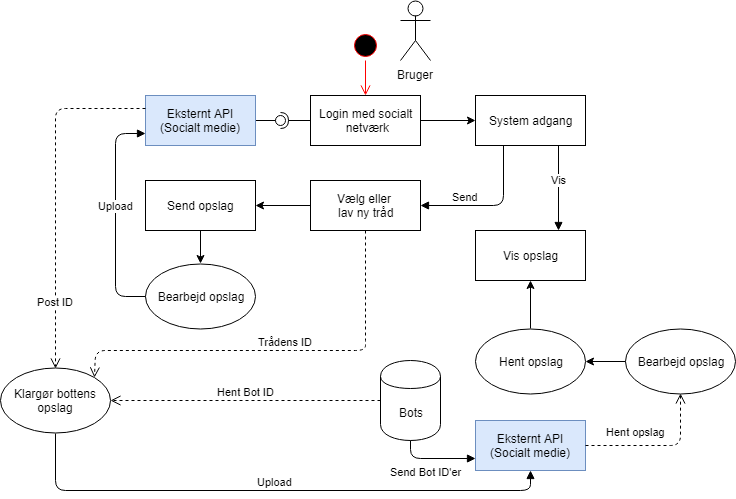
\includegraphics[width=0.8\linewidth]{Projectdoc/Assets/Illustrationer/userbased-system.png}
    \caption{}
    \label{fig:userbased}
\end{figure}
Brugerne logger ind på platformen ved hjælp af deres egne kontooplysninger til et given socialt medie. Platformen har nu mulighed for at sende den hemmelige besked direkte til brugerens egen konto. Platformen lægger automatisk den hemmelige besked ind i den pågældende bruger's opslag, og returnere samtidigt opslagets unikke ID tilbage. Dette ID bliver sammen med et unikt tråd ID 

Det vil sige at brugerne selv har ansvar for at lagre beskeden,


+ Hvis en central BOT bliver undersøgt vil beskederne ikke kunne spores, men mindre de har bottens secret
+ Sammenkædning af posts af samme forfatter

- Ingen løsning til skjul af metadata
- Ekstra requests
- Brugeren kan slette deres posts udenom system, og ødelægge trådens struktur
% - Central server / server cache (Sikkerheds brist)

% Hvordan kan man sikre en fornuftig køre tid? (Undgå 10000 undersøgelser for at finde én kommentar)
% - Formindsk chancen for mistænkelig data trafik. Både i server requests og det visuelt uploaded
% - Load tid

% API udbyderen som brist i systemet?
% - TOS problemer
% - Lukning af bots og dermed samtaler

% Hvordan skal forum strukturen være ? (Design)

% Hvordan kan vi skulle sammenkædnings nødvendig data i metadata?